\section{Housing Stock and Family Space}
\label{app:housing-stock}

This Appendix documents two facts about the housing stock that complement
the event study of Section~\ref{sec:empirical-evidence}: large homes are
mostly owned, and most large owned homes are held by older households.

\subsection{Large homes are owned}

Figure~\ref{fig:tenure-by-size} divides the 2023 housing stock in the
American Housing Survey (AHS) by number of bedrooms and tenure. Of the homes
with four or more bedrooms, 87 percent are owner-occupied and 9 percent are
rented. Of the homes with at most one bedroom, 13 percent are owner-occupied
and 74 percent are rented. In rooms, the unit of the rest of the paper, 43
percent of owner-occupied homes have seven or more rooms, against 7.5
percent of rented homes. The gap holds among families: owners with children
occupy 6.8 rooms on average and renters with children 5.2, and 48.7 percent
of renter households with children live in homes with at most two bedrooms,
against 7.4 percent of owner households with children. These shares describe
the homes households occupy rather than the homes on offer, but they show
that, in the existing stock, a family that wants a large home typically
buys one.

\begin{figure}[t]
\centering
\caption{Tenure of the Housing Stock by Number of Bedrooms (AHS 2023)}
\label{fig:tenure-by-size}
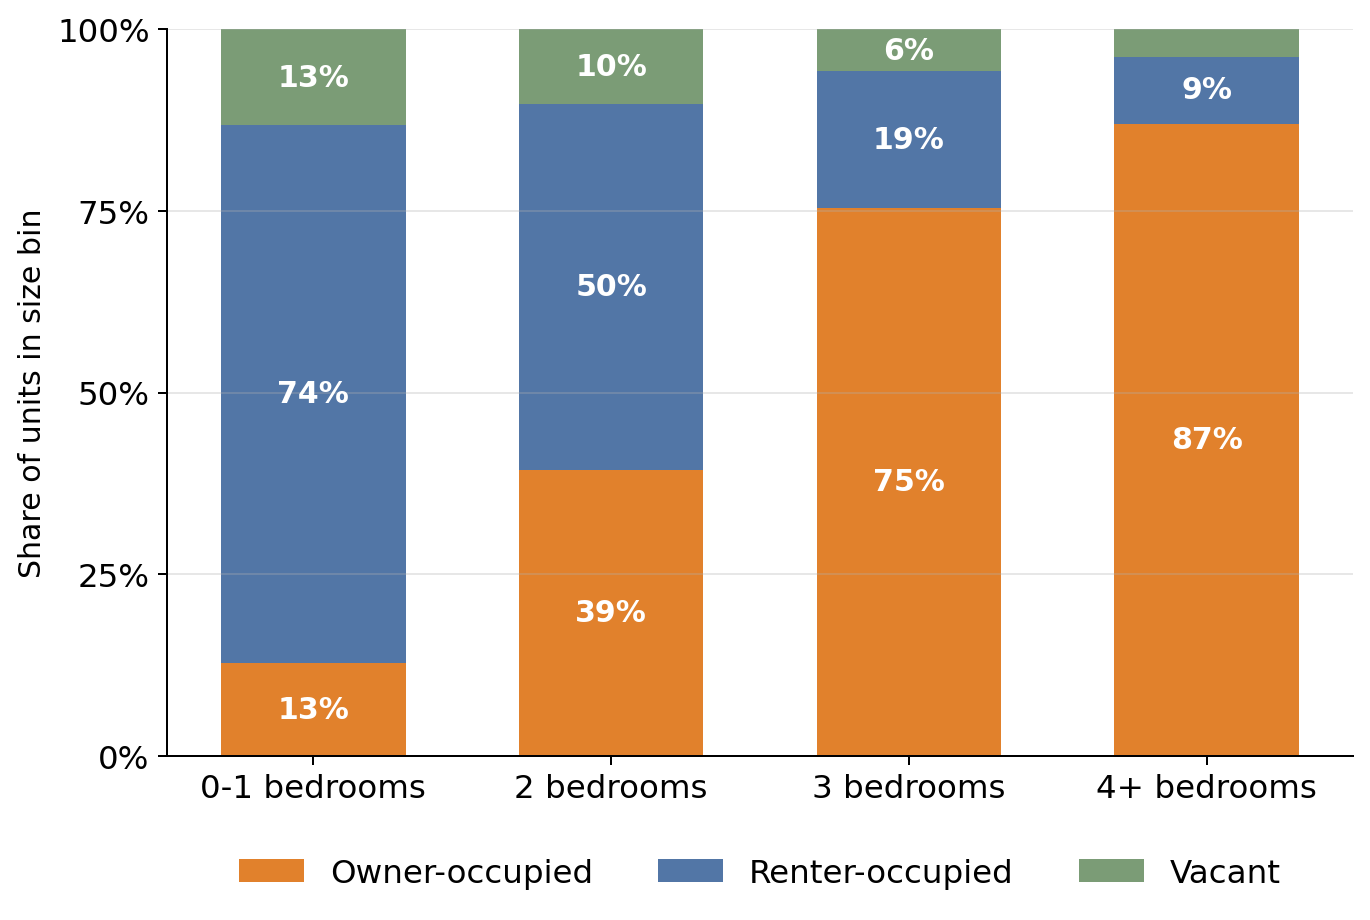
\includegraphics[width=0.62\linewidth]{ahs_tenure_share_within_size}
\par\medskip
\begin{minipage}{0.92\linewidth}
\footnotesize Note: This figure shows the tenure of housing units by number of
bedrooms. Each bar divides the housing units with the
stated number of bedrooms into owner-occupied units, units rented for cash,
and vacant units. Units occupied without payment of cash rent and units whose
occupants have a usual residence elsewhere are excluded. Weighted by the
housing-unit weight. Source: American Housing Survey 2023, national
public-use file.
\end{minipage}
\end{figure}

\subsection{Older households hold the large homes}

Figure~\ref{fig:large-homes} divides the owner-occupied homes with six or
more rooms in 42 large metropolitan areas in the 2023 American Community
Survey (ACS) by the age of the householder and by whether a child of the
householder younger than 18 lives in the home. Households aged 60 to 85
without children at home hold 40.0 percent of these homes, and households
aged 40 to 59 without children at home another 21.8 percent. Households aged
22 to 39 with children hold 10.6 percent. Across all ages, 68.3 percent of
the large owner-occupied homes house no child of the householder, close to
the 72.9 percent of all households in these areas without a child at home.
The large homes are therefore not held disproportionately by households
without children; they are held by the old. I call this concentration the
intergenerational allocation of housing. For a young family, it means that
the existing large homes become available mainly as older households sell
or leave them. The figure says nothing about the price at which older
owners would sell, or about whether young families would have more children
if they held these homes.

\begin{figure}[t]
\centering
\caption{Who Holds the Large Owner-Occupied Homes (ACS 2023)}
\label{fig:large-homes}
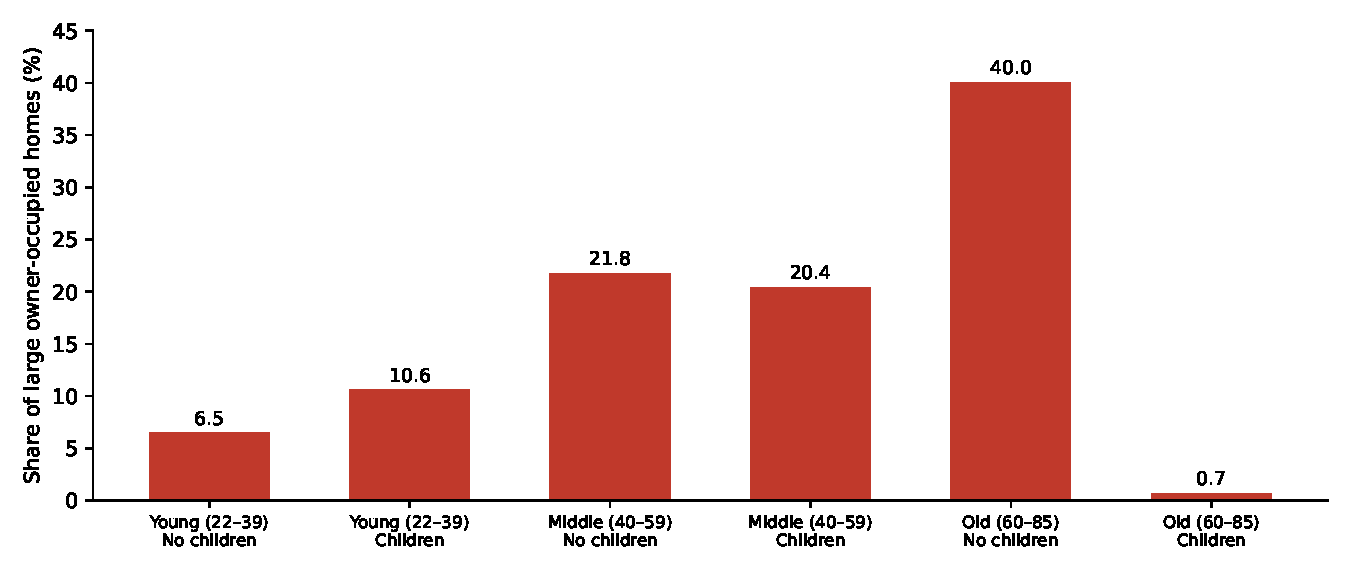
\includegraphics[width=0.9\linewidth]{large_homes_by_age_children_acs2023}
\par\medskip
\begin{minipage}{0.92\linewidth}
\footnotesize Note: This figure shows who holds the large owner-occupied
homes. Each bar is the share of owner-occupied homes
with six or more rooms held by households in the group; the six shares sum to
100 percent. Groups are defined by the age of the householder and by whether
an own child of the householder younger than 18 lives in the household.
Householders aged 22 to 85 in 42 large metropolitan areas, weighted by the
household weight; 289,109 households.
\end{minipage}
\end{figure}

\subsection{Ownership of recent parents}

The same pattern appears in the cross-section. In the 2005--2006 ACS,
household heads aged 30 to 55 whose oldest child is under four are 12.8
percentage points more likely to own than heads without children, a moment
the calibration also targets. Unlike the PSID estimates, this gap compares
different households at a point in time.

\subsection{Data}

The stock facts use the national public-use household file of the 2023
American Housing Survey, weighted by the housing-unit weight. Tenure has three
occupied categories: owned, rented for cash, and occupied without payment of
cash rent. Shares within a tenure use all units of that tenure as the
denominator; the share of seven-plus-room homes that are rented instead uses
all occupied units of that size. It is 8.2 percent when the denominator
contains owned and cash-rented units and 8.1 percent when it also contains
units occupied without cash rent and units with unreported tenure. Bedrooms and
total rooms are different measures. I report bedrooms for comparison with
other work and rooms because rooms are the PSID and ACS outcome and the unit of
the model. Mean rooms among households with children are computed over
households with at least one child present. A cross-section of occupied homes
does not identify the units offered for rent or the choices families would
make at other prices.
